%\documentclass{acm_proc_article-sp}
\documentclass{sig-alternate}

\usepackage{xspace}
\newcommand{\CEU}{\textsc{C\'{e}u}\xspace}
\newcommand{\code}[1] {{\small{\texttt{#1}}}}
\newcommand{\MM}[1] {{\textbf{\texttt{#1}}}}

\usepackage{verbatim}
\usepackage{enumitem}

\usepackage{color}
\definecolor{light}{gray}{0.87}
\definecolor{dark}{gray}{0.30}
%\definecolor{light}{rgb}{.90,.90,.90}
\definecolor{darkgreen}{rgb}{0,.50,0}
\definecolor{darkblue}{rgb}{0,0,.50}
\definecolor{darkred}{rgb}{.50,0,0}
\definecolor{darkpur}{rgb}{.50,0,.50}

% \input bnf.tex

\usepackage{listings}
%\usepackage{textcomp}
\usepackage{url}
\lstset{
%columns=fullflexible,
%basicstyle=\ttfamily,
escapeinside={||},
    %mathescape=true,
    language=C, % choose the language of the code
    basicstyle=\fontfamily{pcr}\selectfont\scriptsize\color{black},
    keywordstyle=\color{black}\bfseries, % style for keywords
    numbers=none, % where to put the line-numbers
    numberstyle=\tiny, % the size of the fonts that are used for the line-numbers
    backgroundcolor=\color{light},
    showspaces=false, % show spaces adding particular underscores
    showstringspaces=false, % underline spaces within strings
    showtabs=false, % show tabs within strings adding particular underscores
    %frame=single, % adds a frame around the code
    tabsize=2, % sets default tabsize to 2 spaces
    %rulesepcolor=\color{gray}
    captionpos=b, % sets the caption-position to bottom
    breaklines=false, % sets automatic line breaking
    %breakatwhitespace=false,
    numbersep=2em,
    % C was used in the blocksworld example to refer to block C and nowhere else
    emph={par,or,hor,do,end,loop,await,emit,input,event,call,with,%
          var,and,then,else,return,pure,deterministic,nohold,finalize,%
          class, every, FOREVER, this, spawn, in, pool, watching, until, 
          interface, each, abort, when, signal, PROC, CHAN, SIGNAL, PAR, not,
          bool, data, tag, escape, new, traverse},
    emphstyle={\bfseries},
    commentstyle=\color{dark}\scriptsize,
    %xleftmargin=20pt,
    %xrightmargin=20pt,
    framesep=20pt,
    %upquote=true,
    %aboveskip={1.5\baselineskip},
}

\begin{document}

\title{Reactive Traversal of Recursive Data Types}
%\subtitle{[Extended Abstract]

\numberofauthors{3}
\author{
\alignauthor
Francisco Sant'Anna \\
    \affaddr{Departamento de Inform\'atica --- PUC-Rio, Brazil} \\
    \email{fsantanna@inf.puc-rio.br}
\alignauthor
Hisham Muhammad \\
    \affaddr{Departamento de Inform\'atica --- PUC-Rio, Brazil} \\
    \email{hisham@inf.puc-rio.br}
\alignauthor
Johnicholas Hines \\
    \affaddr{IDEXX Laboratories} \\
    \email{johnicholas.hines@gmail.com}
}

\maketitle
\begin{abstract}
We propose a structured mechanism to traverse recursive data types 
incrementally, in successive reactions to external input events.
\code{traverse} is an iterator-like anonymous block that can be invoked 
recursively and suspended at any point, retaining the full state and stack 
frames alive.
\code{traverse} is designed for the synchronous language \CEU, inheriting all 
of its concurrency functionality and safety properties, such as parallel 
compositions with orthogonal abortion, static memory management, and bounded 
reaction time and memory usage.
We discuss three applications in the domains of incremental computation and 
control-oriented DSLs that contain reactive and recursive behavior at the same 
time.

\begin{comment}
MIX OF:
\begin{itemize}
    \item recursive calls to anonymous closures
    \item each instance---many co-routines
\end{itemize}

DESIGNED FOR \CEU:
\begin{itemize}
    \item lexical compositions
    \item static memory management
    \item bounded execution/memory
    \item reactive
    \item mutation
\end{itemize}
\end{comment}

\end{abstract}

\category{D.3.3}{Programming Languages}{Language Constructs and Features}

\terms{Design, Languages}

\keywords{Behavior Trees, Domain Specific Languages, Incremental Computation, 
Logo, Recursive Data Types, Structured Programming, Reactive Programming}

\section{Introduction}

\begin{comment}
All examples have working implementations:

- TODO: compare the real code with the listing

\begin{itemize}
\item label "lst.list":               rebls-15/list/list.ceu
\item label "lst.list.sum":           rebls-15/list/list.ceu
\item label "lst.list.sum.react":     rebls-15/list/list.ceu
%
\item label "lst.bt1":                rebls-15/bts-ceu/btree-1.ceu
\item label "lst.bt1.interpreter":    rebls-15/bts-ceu/btree-1.ceu
\item label "lst.bt1.leaf":           rebls-15/bts-ceu/domain-1.ceu
%
\item label "lst.turtle.dsl":         rebls-15/turtle/turtle-2.ceu
\item label "lst.turtle.interpreter": rebls-15/turtle/turtle-2.ceu
\item label "lst.turtle.queue":       rebls-15/turtle/turtle-7.ceu
\end{itemize}
\end{comment}

\begin{comment}
Difficult because of
    multiple stack frames
    concurrent stack frames
    persistent stack frames (across reactions, with other parts executing)
    static memory management
    mutation of the data structure being traversed
\end{comment}

The facilities a given language offers for constructing data types have a 
direct impact on the nature of algorithms that programmers will write on that 
language.
The design of such facilities must take into account the constraints imposed by 
the rest of the language.
As an example, the aim for referential transparency in functional languages 
enforces data structures to be immutable.
Under these constraints, one must then avoid excessive memory copying through 
specialized algorithms~\cite{okasaki.purely}.

In this paper, we discuss the design of recursive data types and an associated
control facility for a language developed under a different set of
constraints. \CEU~\cite{ceu.sensys13,ceu.mod15} is an imperative, concurrent and
reactive language in which the lines of execution, known as \emph{trails},
react all together continuously and in synchronous steps to external stimuli.
Being an imperative language, \CEU features mutable data.
At the same time, it promotes static memory management through lexically-scoped
memory pools, and safe pointer manipulation even under concurrent trails with 
orthogonal abortion~\cite{ceu.mod15}.
These features preclude the availability of general records with arbitrary 
pointers such as \emph{structs} in C.
%Recursive data types in \CEU must, therefore, respect the language's
%memory management guarantees and their use must cope with the synchronous
%concurrency model.

The solution to this problem is twofold, with data and control aspects.
For data management, we introduce a \code{data} type construct with a set of 
restrictions on constructors and assignments that makes static memory 
management possible.
For handling reactive control, we propose a structured mechanism that can 
traverse recursive data types incrementally, in successive reactions to input 
events.
\code{traverse} is an iterator-like anonymous block that can be invoked 
recursively and suspended at any point, retaining the full state and stack 
frames alive.

After we present the design of these constructs, we discuss three applications 
in the domains of incremental computation and control-oriented DSLs.
The applications contain reactive and recursive behavior at the same time and 
showcase the expressiveness of the proposed constructs.
TODO: related/conclusion

\section{C\'eu constructs}

In this section, we present the constructs added to \CEU to support recursive
data types with reactive traversal.

First we present the general flavor of the language with an introductory 
example.
The code in Figure~\ref{lst.intro} defines an input event \code{RESET} (line 
1), a shared variable \code{v} (line 2), and starts two trails with the 
\code{par} construct (lines 3-14): the first (lines 4-8) increments variable 
\code{v} on every second and prints its value on screen; the second (lines 
10-13) resets \code{v} on every external request to \code{RESET}.
\CEU is tightly integrated with \emph{C} and can access libraries of the 
underlying platform directly by prefixing symbols with an underscore (e.g., 
\code{\_printf(<...>)}, in line 7).

In the synchronous model of \CEU, a program reacts to an occurring event 
completely before handling the next.
%
A reaction represents a logical instant in which all trails awaiting the 
occurring event awake and execute, one after the other, until they await again 
or terminate.
%
During a reaction, the environment is invariant and does not interrupt the 
running trails.
If multiple trails react to the same event, the scheduler employs lexical 
order, i.e., the trail that appears first in the source code executes first.
%
For this reason, programs are deterministic even in the presence of side 
effects in concurrent lines of execution.
%
To avoid infinite execution for reactions, \CEU ensures that all loops contain 
\code{await} statements~\cite{ceu.sensys13}.

\begin{figure}[t]
\begin{lstlisting}[numbers=left,xleftmargin=3em]
input void RESET;  // declares an external event
var int v = 0;     // variable shared by the trails
par do
   loop do         // 1st trail
      await 1s;
      v = v + 1;
      _printf("v = %d\n", v);
   end
with
   loop do         // 2nd trail
      await RESET;
      v = 0;
   end
end
\end{lstlisting}
\caption{ Introductory example in \CEU.
\label{lst.intro}
}
\end{figure}

\subsection{Recursive Data Types}

The \code{data} construct in \CEU provides a safer alternative to C's
\code{struct}, \code{union}, and \code{enum} definitions.
%
Figure~\ref{lst.list} illustrates the recursive \code{List} data type,
declared as a tagged union (lines 1--5).
The first tag, \code{NIL} (line 2), represents the empty list and is the 
union's null type.
The second tag, \code{CONS} (line 4), holds a value in the field \code{int 
head} and the rest of the list in the recursive field \code{List tail}.
%
The \code{pool} keyword declares a memory pool of a given size and
a (implicit) reference to its root object.
All memory allocated by \CEU constructs is managed by lexically-scoped memory
pools.

\begin{comment}
A \code{data} entry
declares either a non-recursive structure containing a set of mutable fields
or a tagged union. A tagged union consists of a set of tag declarations, each
of which may be a bare tag or contain mutable fields. If any of the tag
declarations refers to the data type being declared, we have a recursive data
type. In this case, the first tag of the tagged union must be a bare tag, and
it will act as the union's null type: in \CEU, every recursive data type
is an option type.

%% (Uncomment \input bnf.tex above)
\begin{figure}[t]
\begingrammar
<data> : "data" <id> "with" <dataBody> "end" ";"

<dataBody> : <field>* | <tags>

<tags> : <tag> [ "or" <tags> ]* 

<tag> : "tag" <id> \{ ";" | "with" <field>* "end" \}

<field> : "var" <type> <id> ";"

\endgrammar
\caption{
The \code{data} construct in \CEU
}
\end{figure}
\end{comment}

In the first block of the example (lines 7--16), we declare a pool of 
\code{List} objects of size 1 identified by the root reference \code{lst1} 
(line 8), which has the scope limited by the \code{do-end} block (lines 7--16).
The declaration also implicitly initializes the root to the null tag of the 
associated data type (i.e., \code{List.NIL}).
%
Then, we use the \code{=new} construct (lines 9--12), which performs
allocation and assignment: it attempts to dynamically allocate a list of
three elements (10, 20, and 30), inferring the destination memory pool based on 
the assignment's \emph{l-value} prefix (i.e. \code{lst1}).
%
Since the pool has size 1, only the allocation of first element succeeds, with 
the failed allocations returning the null tag (i.e., \code{List.NIL}).
The print command (lines 13--14) outputs ``\texttt{10, 1}'': the \code{head} of 
the first element (the operator \code{`:'} is equivalent to C's \code{`->'}) 
and a true value for the \code{NIL} check of the second element.
%
Finally, the end of the block (line 16) deallocates the pool along with all of 
its elements.

In the second block (lines 18--24), we declare the \code{lst2} pool with an 
unbounded memory limit (i.e., \code{List[]} in line 19).
Now, the three-element allocation succeeds (line 20)%
\footnote{For the sake of brevity, we will omit the data type prefix for tags 
(e.g., \code{List.CONS} becomes \code{CONS}), given that no examples have 
clashes between identifiers.}.
Then, we mutate the tail of the first element to point to a newly allocated 
element in the same pool, which also succeeds (line 21).
In the moment of the mutation, the old subtree (containing values  
``\texttt{20}'' and  ``\texttt{30}'') is completely removed from memory.
The print command (line 22) outputs ``\texttt{50}'', displaying the \code{head}
of the new second element.
%
Again, the end of the block (line 24) deallocates the pool along with all of 
its elements.

%TODO: comment that invalid tag generates runtime error?

% rebls-15/list/list.ceu
\begin{figure}[t]
\begin{lstlisting}[numbers=left,xleftmargin=3em]
data List with
   tag NIL ();
or
   tag CONS (int head, List tail);
end

do
   pool List[1] lst1;
   lst1 = new List.CONS(10,
               List.CONS(20,
                List.CONS(30,
                 List.NIL()));
   _printf("%d, %d\n", lst1:CONS.head,
                       lst1:CONS.tail:NIL);
      // prints 10, 1
end

do
   pool List[] lst2;
   lst2 = new CONS(10, CONS(20, CONS(30, NIL()));
   lst2:CONS.tail = new CONS(50, NIL());
   _printf("%d\n", lst2:CONS.tail:CONS.head);
      // prints 50 (20 and 30 have been freed)
end
\end{lstlisting}
\caption{
A recursive \code{List} data type definition (lines 1--5) with uses (lines 
7--16 and 18--27).
\label{lst.list}
}
\end{figure}

In \CEU, recursive data types have a number of restrictions.
Given that mutations deallocate whole subtrees, data types cannot represent 
general graphs: they must represent tree-like structures.
Elements in different pools cannot be mixed;
and pointers to subtrees (i.e., weak references) must be observed via the
\code{watching} construct, as they can be invalidated at any time
(to be discussed in Section~\ref{sec.traverse}).

%TODO: what kind of structure updates can be made through weak pointers?

\subsection{Traversing Data Types}
\label{sec.traverse}

\CEU introduces a structured mechanism to traverse recursive data types.
The \code{traverse} construct integrates well with the synchronous execution 
model, supporting nested control compositions, such as \code{await} and all 
\code{par} variations.
It also preserves explicit lexical scopes with static memory management.

%We begin by showing the flavor of the construct through an example.
The code in Figure~\ref{lst.list.sum} creates a list (line 1) and traverses it 
to calculate the sum of elements (lines 3--11).
The \code{traverse} block (lines 4--11) starts with the element \code{e} 
pointing to the root of the list \code{lst}.
The \code{escape} statement (lines 6 and 9) returns a value to be assigned to 
the \code{sum} (line 3).
A \code{NIL} list has \code{sum=0} (lines 5--6).
A \code{CONS} list needs to calculate the \code{sum} of its tail recursively, 
invoking \code{traverse} again (line 8), which will create a nested instance of 
the enclosing \code{traverse} block (lines 4--11), now with \code{e} pointing 
to \code{e:CONS.tail}.
%
When used without event control mechanisms, as in this simple example, a 
\code{traverse} block is equivalent to an anonymous closure called recursively.

% rebls-15/list/list.ceu
\begin{figure}[t]
\begin{lstlisting}[numbers=left,xleftmargin=3em]
pool List[3] lst = <...>;  // [10, 20, 30]

var int sum =
   traverse e in lst do
      if e:NIL then
         escape 0;
      else
         var int sum_tail = traverse e:CONS.tail;
         escape sum_tail + e:CONS.head;
      end
   end;

_printf("sum = %d\n", sum);
      // prints 60
\end{lstlisting}
\caption{
Calculating the \emph{sum} of a list.
\label{lst.list.sum}
}
\end{figure}

% TODO: react.ceu with mutation

However, the \code{traverse} construct does not simply amount to an anonymous 
recursive block.
Instead, it takes into account the event system and memory management 
discipline of \CEU.
As such, it is an abstraction defined in terms of more fundamental 
concepts~\cite{ceu.mod15}:
\emph{organisms}, which are objects with their own concurrent trails of 
execution, akin to Simula objects;
and orthogonal abortion, which handles cancellation of trails maintaining 
memory consistency.
%
Figure~\ref{lst.list.sum.react} depicts the expansion of the \code{traverse} 
construct (to be discussed further).

The example in \emph{CODE-1} of Figure~\ref{lst.list.sum.react} extends the 
body of the previous example in Figure~\ref{lst.list.sum} with reactive 
behavior.
%
Now, for each recursive iteration, we print the current \code{head} (line 9) 
and \code{await} 1 second (line 10) before traversing the \code{tail} (line 
11).
%
\CEU enforces at compile time that all accesses to a pointer that cross 
\code{await} statements are protected with an enclosing \code{watching} 
block~\cite{ceu.mod15}.
The \code{watching} aborts its nested block if the referred object is released 
from memory.
%
This ensures that if concurrent side effects affect the pointed object, no code 
uses stale pointers, because the whole block is aborted.
%
With the protection of the \code{watching} block (lines 8--13), if the referred 
element \code{e} (line 8) is released from memory due to a mutation in the list 
during the awaiting period (line 10), we simply ignore the whole subtree and 
return 0 (line 14).

\emph{CODE-2} is the equivalent expansion of \emph{CODE-1} without the 
\code{traverse} construct.
The body of the \code{traverse} (lines 5--15 of \emph{CODE-1}) is abstracted in 
the body of the \code{Frame} class (lines 3--26 of \emph{CODE-2}), which is 
analogous to a ``stack frame'' of a programming language with subroutines.
Likewise, the \code{pool} of frames (line 28 of \emph{CODE-2}) is analogous to 
a runtime ``call stack''.
We limit the number of stack frames to match the maximum number of elements to 
traverse (line 1 of \emph{CODE-1} and lines 1,28 of \emph{CODE-2}).
Therefore, to ``call'' the first \code{traverse} iteration, we dynamically 
\code{spawn} a \code{Frame} instance into the \code{frames} pool (lines 29--30 
of \emph{CODE-2}).
Then, we immediately \code{await} the termination of this \code{frame}, which 
is in the lowest level of the ``call stack'', i.e., only after the 
\code{traverse} rolls back and clears the ``call stack'' that we acquire the 
\code{sum} and print it (line 31--34 of \emph{CODE-2}).

A \code{Frame} receives three arguments in the constructor (lines 4--6 of 
\emph{CODE-2}:
a reference to a \code{pool}, to recursively \code{spawn} new frames;
a reference to its parent frame, to handle abortion;
and a pointer to the subtree of the data type, to be able to manipulate it.
%
The \code{Frame} constructor for the first ``call'' (lines 29--30 of 
\emph{CODE-2}) receives the static pool of frames, the running organism as the 
parent (i.e., \code{this}), and the tree of the data type passed to the 
original \code{traverse} (line 4 of \emph{CODE-1}).
%
The \code{Frame} constructor for recursive ``calls'' (lines 15--18 of 
\emph{CODE-2}) receives the same pool of frames, the current ``stack frame'' as 
parent, and the subtree of the data type passed to the original recursive 
\code{traverse} invocation (line 11 of \emph{CODE-1}).

The \code{Frame} body (lines 8--25 of \emph{CODE-1}) always aborts with the
\code{parent} frame termination.
Given that a \code{traverse} body can execute (and terminate) trails running 
concurrently with the recursive invocation, the enclosing \code{watching} 
guarantees that the hierarchy in the ``call stack'' will be preserved (i.e., 
that there are no orphan frames executing).
%
The remaining code is almost the same in the original \code{traverse} body and 
in the \code{Frame} body (lines 5--15 of \emph{CODE-1} and lines 9--23 of 
\emph{CODE-2}).
The only exception is the recursive invocation of the \code{traverse} (line 11 
of \emph{CODE-1}), which expands to a \code{spawn} of a \code{Frame} (lines 
15--18 of \emph{CODE-2}) with similar behavior to the first invocation (lines 
29--30 of \emph{CODE-2}).

As the expansion illustrates, three aspects make \code{traverse} fundamentally 
different from an recursive function calls:
%
\begin{enumerate}
\item Each \code{traverse} invocation spawns a new organism which can execute 
concurrently with other parts of the application.
Also, each organism itself can invoke multiple concurrent trails, adding more 
complexity in comparison to standard functions~\cite{ceu.mod15}.
%
\item Traversal is declared in terms of a specific lexically-scoped memory pool 
for a data structure.
Therefore, we can infer at compile time the maximum traversal depth if the data 
is bounded (e.g., \code{List[3] lst}).
Enforcing execution limits is an important requirement for constrained and 
real-time embedded systems, which is the original application domain of 
\CEU~\cite{ceu.sensys13}.
In addition, given that the pool of frames is expanded in the same lexical 
scope, when the data goes out of scope, all stack frames are automatically 
aborted~\cite{ceu.mod15}.
%
\item The execution body of a \code{traverse} block is implicitly wrapped by a 
concurrency construct that watches for mutations of the current node.
In practice, this means that it reacts consistently if another trail of 
execution modifies the data structure being traversed.
\end{enumerate}

We believe that the \code{traverse} construct, more than a simple convenience, 
considerably reduces the complexity of programs, handling a complex hierarchy 
of behaviors associated with recursive data types automatically.

%TODO: expansion is simplified:
% option type, mem fail, passing arguments, outer closure

\begin{figure*}[t]
\begin{minipage}[t]{0.48\linewidth}
% rebls-15/list/list.ceu
\begin{lstlisting}[numbers=left,xleftmargin=3.5em,title=CODE-1: Original code (with \code{traverse})]
pool List[3] lst = <...>;  // [10, 20, 30]

var int sum =
   traverse e in lst do
      if e:NIL then
         escape 0;
      else
         watching e do
            _printf("me = %d\n", e:CONS.head);
            await 1s;
            var int sum_tail = traverse e:CONS.tail;
            escape sum_tail + e:CONS.head;
         end
         escape 0;
      end
   end;

_printf("sum = %d\n", sum);
      // prints 60














.
\end{lstlisting}
\end{minipage}
%
\begin{minipage}[t]{0.52\linewidth}
\begin{lstlisting}[numbers=left,xleftmargin=3.5em,title=CODE-2: Expanded code (without \code{traverse})]
pool List[3] lst = <...>;  // [10, 20, 30]

class Frame with
   pool Frame[3]& frames;
   var  Frame&    parent;
   pool List[3]*  e;
do
   watching this.parent do
      if e:NIL then
         escape 0;
      else
         watching e do
            _printf("me = %d\n", e:CONS.head);
            await 1s;
            var Frame* frame = spawn Frame(this.frames,
                                           this,
                                           &e:CONS.tail);
                               in this.frames;
            var int sum_tail = await *frame;
            escape sum_tail + e:CONS.head;
         end
         escape 0;
      end
   end
   escape 0;
end

pool Frame[3] frames;
var Frame* frame = spawn Frame(frames, this, &lst)
                   in frames;
var int sum = await *frame;

_printf("sum = %d\n", sum);
      // prints 60
\end{lstlisting}
\end{minipage}
%
%\rule{17.5cm}{0.37pt}
\caption{
Calculating the \emph{sum} of a list, one element each second.
The \code{traverse} construct is a syntactic sugar that can be ``desugared'' 
with explicit organisms.
\label{lst.list.sum.react}
}
\end{figure*}

\begin{comment}
\CEU can also ensure termination for \code{traverse}
% construct can also enforce bounded execution time, by performing a limited 
% number of steps, each of them in a separate synchronous reaction.
%This can be asserted
by verifying that the structure of the
recursive steps converge to the base cases, or by limiting the maximum number 
of recursive invocations based on the size of the data type pool.
If a pool is limited to at most \emph{N} elements, then you can have at most 
\emph{N} alive \code{traverse} bodies.
Enforcing execution limits is an important requirement for
constrained and real-time embedded systems, which is the original application
domain of \CEU~\cite{ceu.sensys13}.

% TODO: abstract fold example?
% TODO: or mention that is not the focus here
% TODO: or mention that abstractions will be used in the applications
\begin{figure}[t]
\begin{lstlisting}[numbers=left,xleftmargin=3em]
class FoldL with
   pool List[]&   lst;
   pool Action[]& actions;
   var  int&     acc;
do
   traverse e in lst do
      if e:CONS then
         var Action*? a =
            spawn Action(e, acc);
         await *a;
      end
   end
end
\end{lstlisting}
%\rule{8.5cm}{0.37pt}
\caption{
Calculating the \emph{sum} of a list.
\label{lst.sum}
}
\end{figure}
\end{comment}

\section{Applications}

In this section, we present three applications that explore the reactive and 
incremental nature of the \code{traverse} construct.
We start with standard \emph{Behavior Trees} used in video games for AI 
modeling~\cite{isla2005,hecker2009my}.
Then, we show a \emph{Logo Turtle}~\cite{papert.logo} that can execute commands 
in parallel (e.g., \code{move} and \code{rotate}).
Finally, we extend the Turtle example with a dynamic and concurrent queue of 
commands that can affect the running program.

\subsection{Behavior Trees}

\emph{Behavior Trees} are a family of DSLs used for game AI.
The term is loose, because different games use different languages.
For our purposes it indicates an interpreted domain-specific language
for concurrent creature behavior that includes sequence and selection combinators.

The \code{SEQ} can be understood as short-circuit evaluation of an `and',
while the \code{SEL} corresponds to an `or'.
This skeleton is extensible with leaves to test properties, set properties, 
perform animations and sounds, etc., and is an effective alternative to finite 
state machines for authoring game AI.
%
However, because the evaluation of each tree extends across many frames, 
writing behavior tree nodes and leaves in other languages is an exercise in 
stack-ripped event-driven programming~\cite{krohn2007events}.
%
%and there are sufficiently many creatures that it is infeasible for each 
%creature to have its own thread,
%
By lowering the barrier to writing custom nodes and leaves, \CEU lightweight 
event control mechanisms make behavior trees more usable.

Figure~\ref{lst.bt1} describes a generic grammar for behavior trees (lines 
1--9).
The \code{SEQ} and \code{SEL} tags (lines 4 and 6) are recursive and behave as 
described above.
The \code{LEAF} tag (line 8) receives a reference to a \code{Leaf} organism, 
which is defined externally and implements the behavior for the domain-specific 
application.
%
The interpreter for tree instances is abstracted in a class definition (lines 
11--37), which receives the tree to execute as an argument (line 12), acquires 
the return status of the traversal (line 14) and returns it as its final result 
(lines 36).
%
The traversal takes into account the semantics of the composite nodes.
%
For the \code{SEQ} tag (lines 16--22), we traverse the \code{first} subtree 
(line 17) and only if it succeeds, we traverse the \code{second} subtree (line 
21).
%
For the \code{SEL} tag (lines 23--29), we traverse the \code{first} subtree 
(line 24) and only if it fails, we traverse the \code{second} subtree (line 
28).
%
Finally, the \code{LEAF} tag does the real work and is domain specific.
The \code{do Class} syntax (line 31--32) creates an anonymous and lexically 
scoped organism of the referred class and awaits its termination.
The organism itself can contain any valid code in \CEU and execute for an 
arbitrary amount of time~\cite{ceu.mod15}.
The tree traversal hangs and waits for its return status (line 33).
This is the expected behavior given that \code{SEQ} and \code{SEL} nodes want 
to execute their children in sequence.

% rebls-15/bts-ceu/btree-1.ceu
\begin{figure}[t]
\begin{lstlisting}[numbers=left,xleftmargin=3em]
data BTree with
   tag NIL ();
or
   tag SEQ (BTree first, BTree second);
or
   tag SEL (BTree first, BTree second);
or
   tag LEAF (Leaf& leaf);
end

class BTreeInterpreter with
   pool BTree[]& btree;
do
   var int ret =
      traverse t in btree do
         if t:SEQ then
             var int ok = traverse t:SEQ.first;
             if ok == 0 then
                 escape ok;
             end
             ok = traverse t:SEQ.second;
             escape ok;
         else/if t:SEL then
             var int ok = traverse t:SEL.first;
             if ok != 0 then
                 escape ok;
             end
             ok = traverse t:SEL.second;
             escape ok;
         else/if t:LEAF then
            var int ret =
                do Leaf(t:LEAF.leaf);
            escape ret;
         end
      end;
   escape ret;
end
\end{lstlisting}
\caption{
A simple generic grammar of behavior trees with \emph{sequence} and 
\emph{selector} composite nodes with a straightforward interpreter.
\label{lst.bt1}
}
\end{figure}

The blocks world is a classical planning domain~\cite{slaney2001blocks}.
The leaves of a behavior tree in an extended blocks world domain
might include sensor leaves that either succeed or fail,
as well as actuator leaves that move blocks and unconditionally succeed.
The tree in Figure~\ref{lst.bt1.example} is based on output from Contingent-FF~\cite{hoffmann2005contingent},
and the blocks domain extended with sensor actions is one of Contingent-FF's benchmark problems.

In this case, we have somehow pinned down the
situation to two possibilities.
%
We use a \code{SEL} node and a sensor leaf to decide which strategy is appropriate,
and \code{SEQ} nodes and actuator leaves to execute it.
This illustrates how the behavior tree can exhibit goal-directed behavior.
The goal-directedness is not automatic; rather, behavior trees are authored
by designers to exhibit goal-directedness.
The \code{traverse} feature allows runtime-authored behavior, 
which is one of the crucial features of behavior trees.
Alternatively, \code{traverse} allows \CEU to
to consume at runtime the output of CPU-intensive algorithms such as planners.

\begin{figure}[t]
\begin{lstlisting}[numbers=left,xleftmargin=3em]
pool BTree[] btree = new SEQ(SEL(SEQ(
      LEAF(SENSE_ON_TABLE(C)),
      LEAF(MOVE_BLOCK_TO_BLOCK(B, C, A))),
    SEQ(
      LEAF(MOVE_TO_TABLE(C, B)),
      LEAF(MOVE_FROM_TABLE(B, A)))),
  LEAF(MOVE_FROM_TABLE(C, B)));
\end{lstlisting}
\centerline{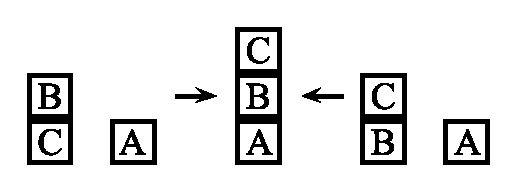
\includegraphics[scale=0.5]{blocksworld.eps}}
%\rule{8.5cm}{0.37pt}
\caption{ A blocks world behavior tree.
If C is on the table,
then we move B from C to A,
and C from the table to B,
achieving an ABC stack.
But if C is not on the table,
we move C from B to the table,
B from the table to A,
and C from the table to B,
also achieving an ABC stack.
\label{lst.bt1.example}
}
\end{figure}

\subsection{Logo Turtle}

Our second example is an interpreter for a simple variant of the classic Logo
turtle-graphics interpreter \cite{papert.logo}.
The aim of this example is to demonstrate parallel traversal.
In our variant, we can instruct the turtle to move and rotate in parallel, 
tracing curves.

% We declare a data type which defines our abstract syntax, with each tag 
% representing one of the supported Logo commands. A tree of nodes represents a 
% program, and the interpreter is implemented as a traversal of this tree.

Figure~\ref{lst.turtle} presents the data type \code{Command} (lines 1--9), 
which specifies the abstract syntax of our Logo variant.
As in traditional Logo, commands can execute in sequence through the \code{SEQ} 
tag (line 4), and can also repeat a number of times through the \code{REPEAT} 
tag (line 6).
%
Our variant extends the \code{MOVE} and \code{ROTATE} commands to take as 
arguments the speed at which they should affect the turtle (lines 8 and 12).
For example, a \code{Command.MOVE(300)} node directs the turtle to move at the 
speed of 300 pixels per second, indefinitely.
%
Therefore, the only way to make the turtle stop moving or rotating is through 
two \CEU-like extensions added to our Logo variant:
The \code{AWAIT} tag (line 12) simply awaits a given number of milliseconds.
The \code{PAROR} tag (line 14), modeled after the \CEU construct \code{par/or},
launches two commands in parallel, and aborts both of them as soon as one of
them finishes.
%
As an example, the program in Figure~\ref{lst.turtle.example} makes the turtle 
to move along a semicircle.

The interpreter for the commands is also abstracted in a class definition 
(lines 17--52 of Figure~\ref{lst.turtle}).
%
It holds as attributes a reference to a \code{Turtle} object (which implements 
the UI) and reference to the commands (lines 18--19).
The execution body of the class uses the \code{traverse} construct to interpret 
the commands (lines 21--51).
%
The \code{SEQ} tag (lines 23--25) traverses each of its child commands in 
sequence (in contrast with the \code{BTreeInterpreter}, it does not handle 
failures).
%
The \code{REPEAT} tag (lines 27--30) traverses its command the specified number 
of times.
%
The \code{MOVE} and \code{ROTATE} tags (lines 32--34 and 36--38) relies on 
predefined classes of organisms to update the position and orientation of the 
\code{turtle} received as argument in the constructor (line 18).
%
The \code{AWAIT} tag (lines 40--41) simply causes the current trail of 
execution of the interpreter to await the given amount of time.
%
Finally, the \code{PAROR} tag (lines 40--48) uses the \code{par/or} construct
to traverse both subcommands at the same time. As per the semantics of
\code{par/or}, as soon as one of the subtrees terminate its execution,
the other one is aborted.

Note that the entire interpreter block is surrounded by a \code{watching}
construct (line 22).
As discussed in Section~\ref{sec.traverse}, the \CEU compiler enforces the 
presence of a guard, due to the use of the \code{cmd} pointer in code that 
spans multiple reactions. This ensures clean abortion in case the AST is 
mutated by code running other trails.

% rebls-15/turtle/turtle-2.ceu
% rebls-15/turtle/turtle-7.ceu
\begin{figure}[t]
\begin{lstlisting}[numbers=left,xleftmargin=3em]
data Command with
   tag NOTHING ();
or
   tag SEQ (Command first, Command second);
or
   tag REPEAT (int times, Command command);
or
   tag MOVE (int pixels);
or
   tag ROTATE (int angle);
or
   tag AWAIT (int ms);
or
   tag PAROR (Command first, Command second);
end

class CommandInterpreter with
   var  Turtle&    turtle;
   pool Command[]* cmds;
do
   traverse cmd in cmds do
      watching cmd do
         if cmd:SEQ then
            traverse cmd:SEQ.first;
            traverse cmd:SEQ.second;

         else/if cmd:REPEAT then
            loop i in cmd:REPEAT.times do
               traverse cmd:REPEAT.command;
            end

         else/if cmd:MOVE then
            do TurtleMove(turtle,
                          cmd:MOVE.pixels);

         else/if cmd:ROTATE then
            do TurtleRotate(turtle,
                            cmd:ROTATE.angle);

         else/if cmd:AWAIT then
            await (cmd:AWAIT.ms) ms;

         else/if cmd:PAROR then
            par/or do
               traverse cmd:PAROR.first;
            with
               traverse cmd:PAROR.second;
            end
         end
      end
   end
end
\end{lstlisting}
\caption{ DSL grammar and interpreter for a Logo turtle.
\label{lst.turtle}
}
\end{figure}

\begin{verbatim}
\end{verbatim}
\begin{figure}[t]
\begin{lstlisting}[numbers=left,xleftmargin=3em]
pool Command[] cmds =
   new PAROR(
         AWAIT(1000),
         PAROR(MOVE(300), ROTATE(180)));

var Turtle turtle;
do CommandInterpreter(turtle, cmds);
\end{lstlisting}
%\rule{8.5cm}{0.37pt}
\caption{ A turtle program.
\label{lst.turtle.example}
}
\end{figure}

\subsection{Enqueuing Commands}
\label{sub.enqueuing}

All examples so far create a fixed tree that does not vary during traversal.
%
Figure~\ref{lst.turtle.queue} extends the Turtle application with a queue of 
pending commands to execute after the running commands terminate.

We define a new \code{Queue} data type in (\emph{CODE-3}):
\code{ROOT} has a \code{running} subtree with the running commands, a 
\code{waiting} queue of pending commands to execute, and a \code{tmp} node that 
allows in-place manipulation of the tree.
Given that all newly allocated nodes must reside in a pool, the \code{tmp} node 
represents a pointer TODO.
\code{ITEM} represents a queue item and contains a \code{cmd} subtree with the 
command to execute, and a \code{prv} queue item pointing to an older item that 
should execute first (i.e., the queue is in reverse order).
%
We define a new \code{Queue} data type in \emph{CODE-3}:
The tag \code{ROOT} has a \code{runnning} subtree with the running commands, a 
\code{waiting} queue of pending commands to execute afterwards, and a 
\code{tmp} node to allows in-place manipulation of the tree (to be discussed 
further).
%
The \code{ITEM} tag represents a queue item and contains a \code{cmds} subtree 
with the commands to execute, and a \code{prv} queue item pointing to an older 
item that should execute first (i.e., the queue is in reverse order).
%
As Figure~\ref{fig.queue-1} illustrates in box \code{0}, a queue instance 
should have a single \code{ROOT} node with linked lists of \code{ITEM} nodes in 
the \code{running} and \code{waiting} fields.
Except on command creation, the \code{tmp} field is always \code{NIL}.

The \code{queue} traversal in \emph{CODE-4} handles the tags \code{ROOT} (lines 
3--16) and \code{ITEM} (lines 17--20).
%
The \code{ROOT} traversal is a continuous \code{loop} that executes the 
\code{running} subtree and swaps it on termination with the \code{waiting} 
queue.
The \code{par/and} (lines 5--9) ensures that that the swap only occurs after 
the current \code{running} commands terminate (line 6) \emph{and} something (in 
parallel) mutates the \code{waiting} subtree (line 8), meaning that the queue 
is no longer empty.
The swapping process (lines 10--15) is illustrated in Figure~\ref{fig.queue-1} 
in the respective boxes (0--2):
%
\begin{enumerate}[start=0]
%
\item The initial state assumes pre-existing \code{running} and \code{waiting} 
items.
\item Lines 10--11 assign the \code{waiting} subtree to the \code{running} 
field (mark~\MM{(a)}), releasing the old subtree (mark~\MM{(b)})).
The \code{waiting} field is automatically set to \code{NIL} (mark~\MM{(c)}).
%
\item Lines 12--15 assign a new neutral \code{ITEM} (with a dummy 
\code{NOTHING} command in the \code{cmds} field) to the \code{waiting} queue 
(mark~\MM{(d)}).
%
\end{enumerate}
%
After the swapping process, the \code{loop} restarts and traverses the new 
\code{running} commands.
%
The \code{ITEM} traversal is straightforward:
first we traverse the previous item (line 18), and then we reuse the 
\code{CommandInterpreter} class of Figure~\ref{lst.turtle} to traverse the 
commands (line 19--20).

Even though this example mutates the \code{running} field only \emph{after} its 
traversal terminates, it is safe to do an arbitrary mutation at any time.
Note that the compiler enforces the use of the \code{watching} construct (lines 
3--22) to enclose the running turtle interpreter (lines 19--20).
Hence, if its enclosing \code{ITEM} (line 17) is mutated, the \code{watching} 
will awake and abort the interpreter inside its lexical scope.

The enqueuing of new commands is depicted in \emph{CODE-5}.
The external input event \code{ENQUEUE} (line 1) accepts \emph{move} and 
\emph{rotate} commands with an associated velocity and time (i.e., 
\code{char*,int,int} arguments).
The \code{every} loop reacts to each occurrence of \code{ENQUEUE}, creating and 
enqueuing the requested command, as illustrated in Figure~\ref{fig.queue-2} 
(1--3):
%
\begin{enumerate}[start=0]
%
\item The initial state assumes the pre-existing neutral \code{ITEM} in the 
root of the \code{waiting} field.
%
\item Line 4--9 create the new \code{ITEM}, with the set of commands to 
\code{MOVE} the turtle, and assigns it to the \code{tmp} field (mark~\MM{a}).
%
\item Lines 13--14 move the already \code{waiting} commands to tail of the 
\code{tmp} node (mark~\MM{(b)}).
Note that the neutral \code{ITEM} is skipped to avoid the \code{waiting} root 
to become \code{NIL} and awake the \code{ROOT} node (line 8 of \emph{CODE-4}) 
before we finish the enqueuing operation.
The old location for the moved commands is automatically set to \code{NIL} 
(mark~\MM{(c)}).
%
\item Line 15 moves the \code{tmp} subtree back to the \code{waiting} field 
(mark~\MM{(d)}), releasing the neutral \code{ITEM} (mark~\MM{(e)}), and 
notifying the \code{ROOT} node that the queue is no longer empty.
The \code{tmp} field is automatically set to \code{NIL} (mark~\MM{(f)}).
%
\end{enumerate}
%

- TODO: modularization of data type and travesal

\begin{figure*}[t]
\begin{minipage}[t]{0.22\linewidth}
\begin{lstlisting}[title=CODE-3: \code{Queue} type]
data Queue with
  tag NIL ();
or
  tag ROOT (Queue running,
            Queue waiting,
            Queue tmp);
or
  tag ITEM (Command cmds,
            Queue prv);
end










.
\end{lstlisting}
\end{minipage}
%
\begin{minipage}[t]{0.36\linewidth}
\begin{lstlisting}[numbers=left,xleftmargin=3.5em,title=CODE-4: Queue traversal]
traverse qu in queue do
  watching qu do
    if qu:ROOT then
      loop do
        par/and do
          traverse qu:ROOT.running;
        with
          await qu:ROOT.waiting;
        end
        qu:ROOT.running =
          qu:ROOT.waiting;
        qu:ROOT.waiting =
          new ITEM(NOTHING(), NIL());
      end
    else/if qu:ITEM then
      traverse qu:ITEM.prv;
      do CommandInterpreter(
            turtle, qu:ITEM.cmds);
    end
  end
end
\end{lstlisting}
\end{minipage}
%
\begin{minipage}[t]{0.39\linewidth}
\begin{lstlisting}[numbers=left,xleftmargin=3.5em,title=CODE-5: Enqueuing commands]
input (char*,int,int) ENQUEUE;
every (cmd,vel,time) in ENQUEUE do
  if _strcmp(cmd,"move")==0 then
    queue.ROOT.tmp =
      new ITEM(
            PAROR(
              MOVE(vel),
              AWAIT(time)),
            NIL());
  else/if _strcmp(cmd,"rotate")==0 then
    <...> // analogous to the MOVE above
  end
  queue.ROOT.tmp.ITEM.prv =
    queue.ROOT.waiting.ITEM.prv;
  queue.ROOT.waiting = queue.ROOT.tmp;
end




.
\end{lstlisting}
\end{minipage}
%
%\rule{17.5cm}{0.37pt}
\caption{ Queue extension for the Turtle DSL of
          Figure~\ref{lst.turtle}.
\label{lst.turtle.queue}
}
\end{figure*}

\begin{figure*}[t]
\begin{minipage}[t]{0.33\linewidth}
\centering
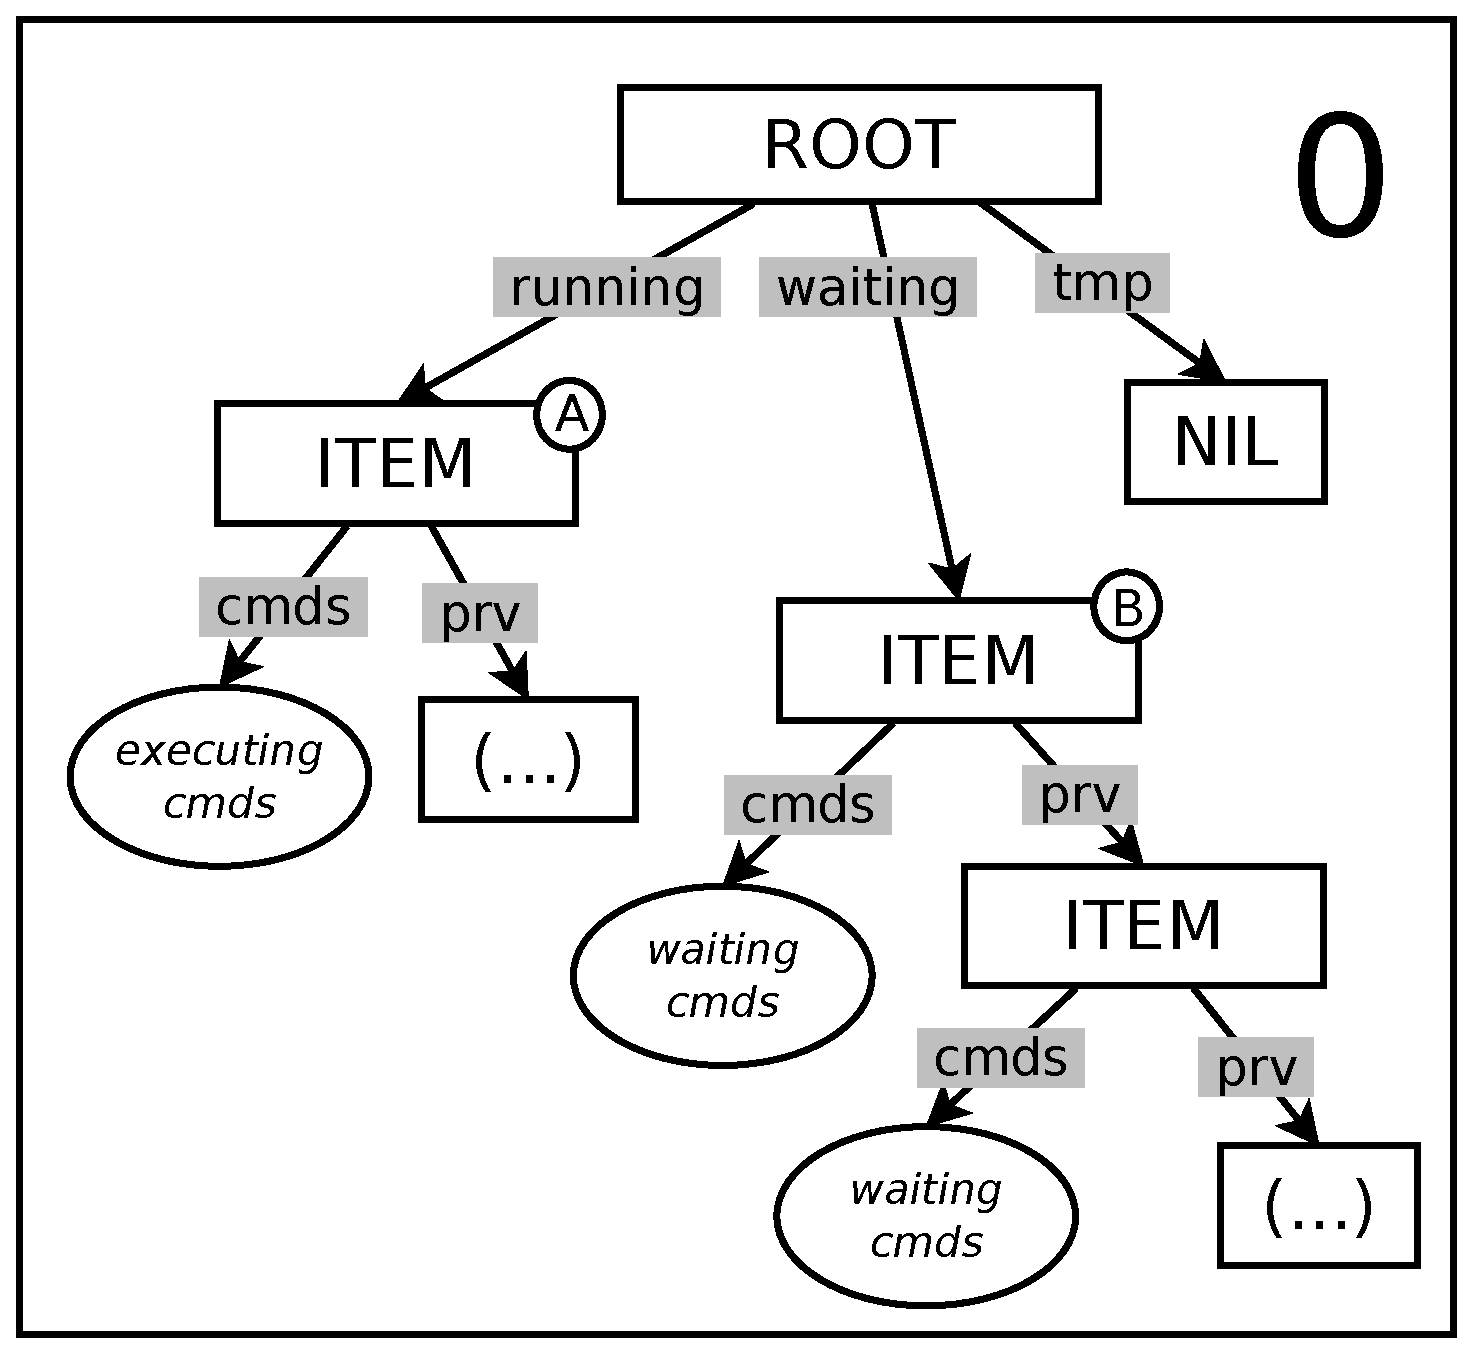
\includegraphics[scale=0.23]{queue-10.eps}
\end{minipage}
\begin{minipage}[t]{0.33\linewidth}
\centering
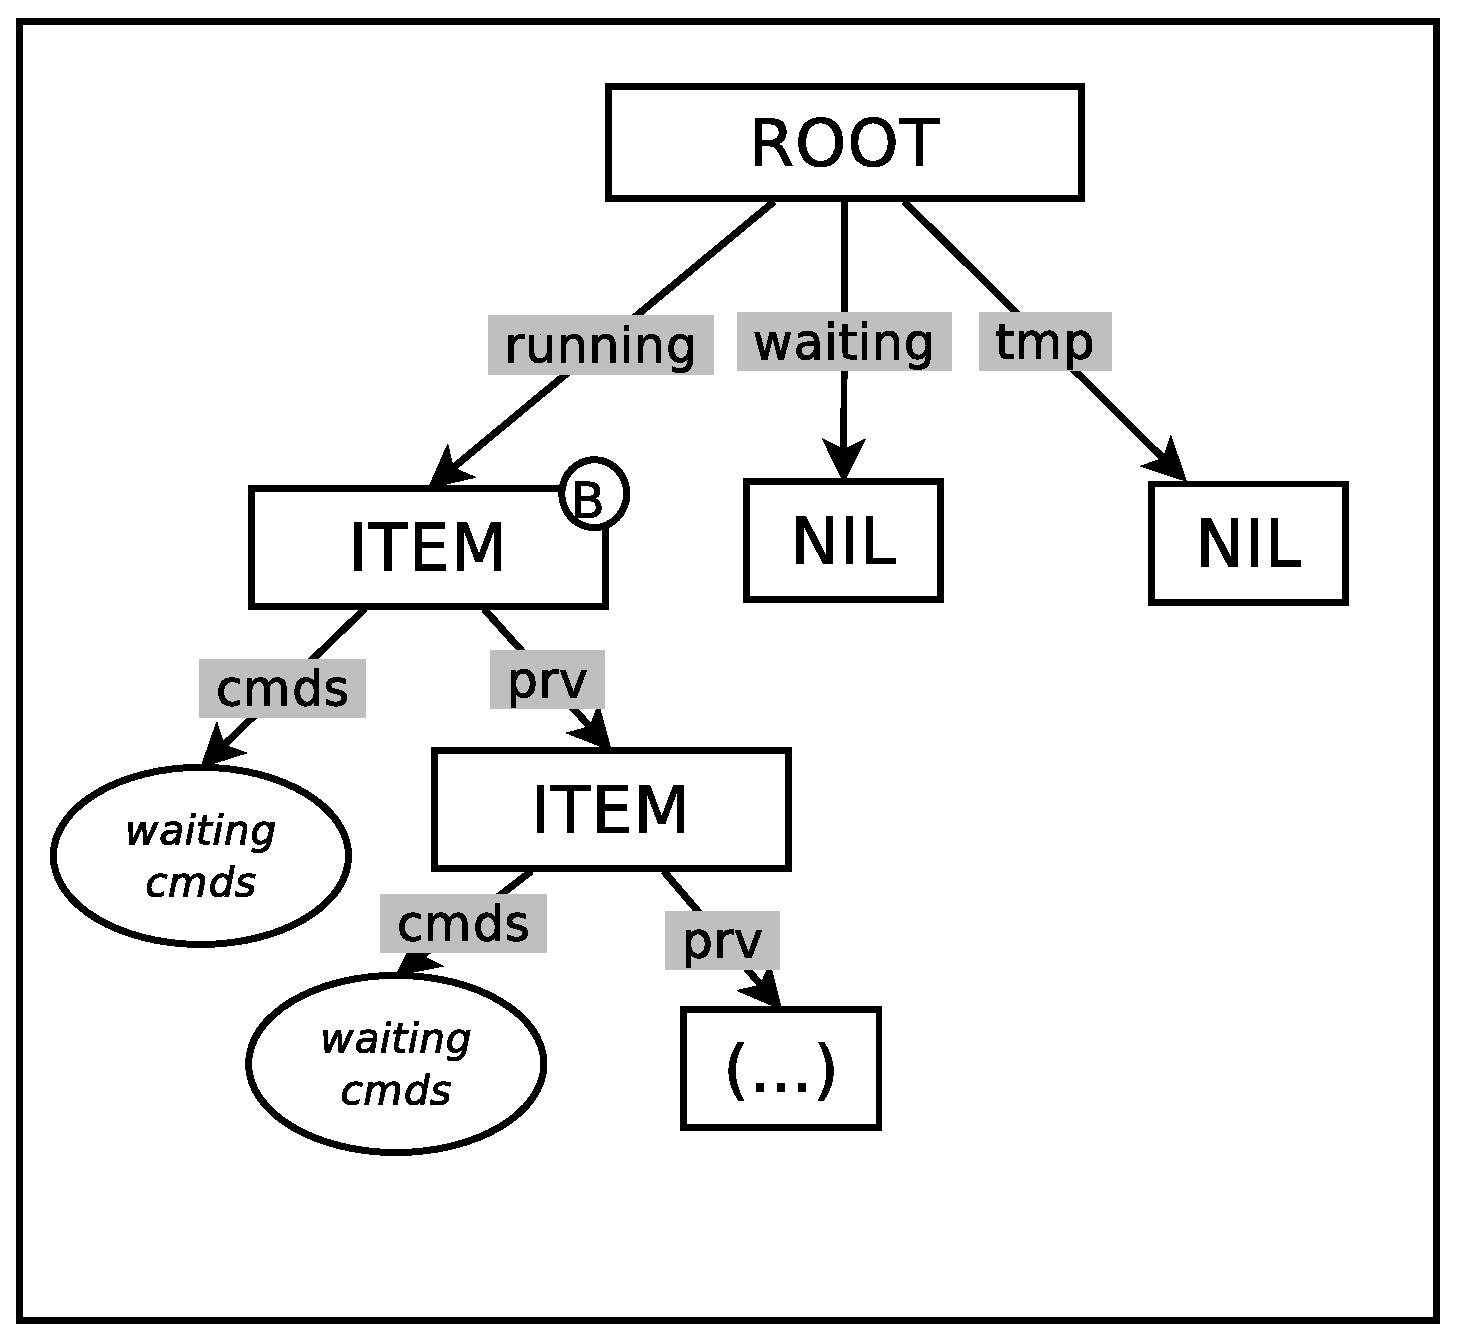
\includegraphics[scale=0.23]{queue-11.eps}
\end{minipage}
\begin{minipage}[t]{0.33\linewidth}
\centering
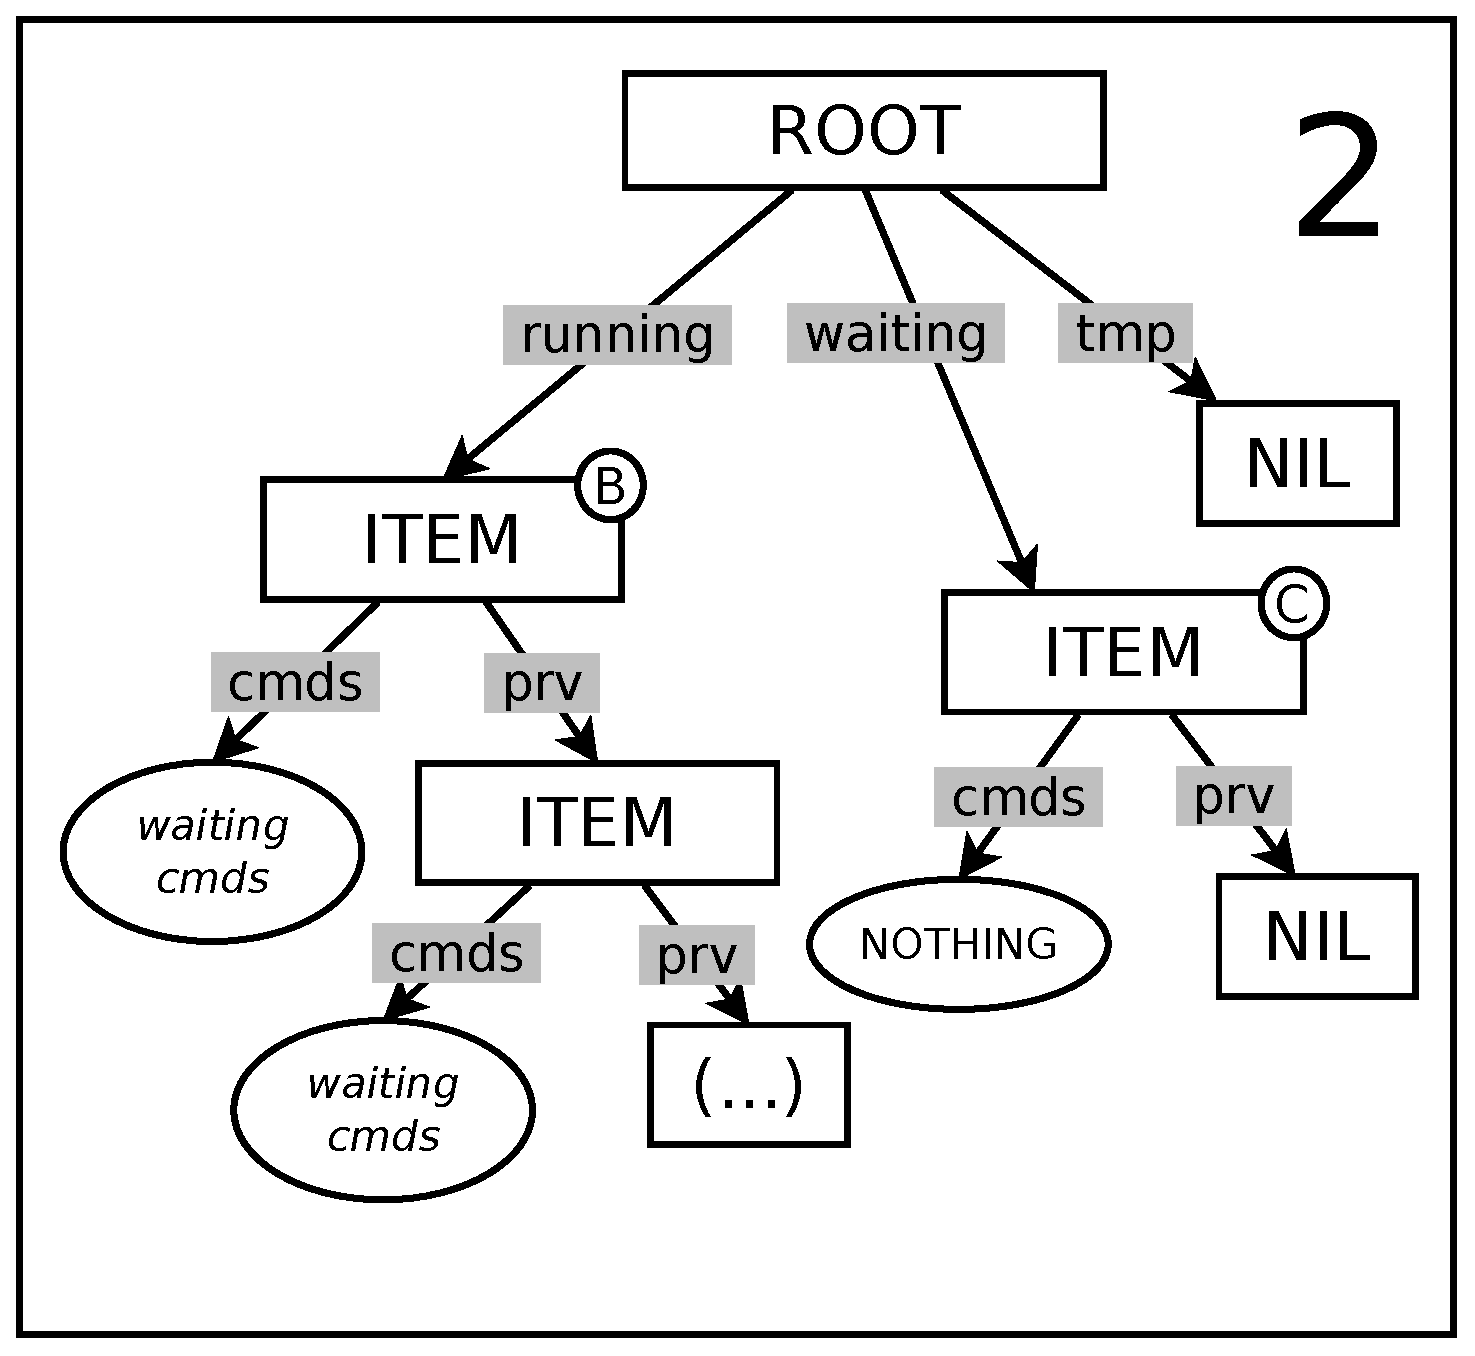
\includegraphics[scale=0.23]{queue-12.eps}
\end{minipage}
\caption{
Swapping \code{waiting} and \code{running} commands.
\label{fig.queue-1}
}
\end{figure*}

\begin{figure}[t]
\begin{minipage}[t]{0.99\linewidth}
\centering
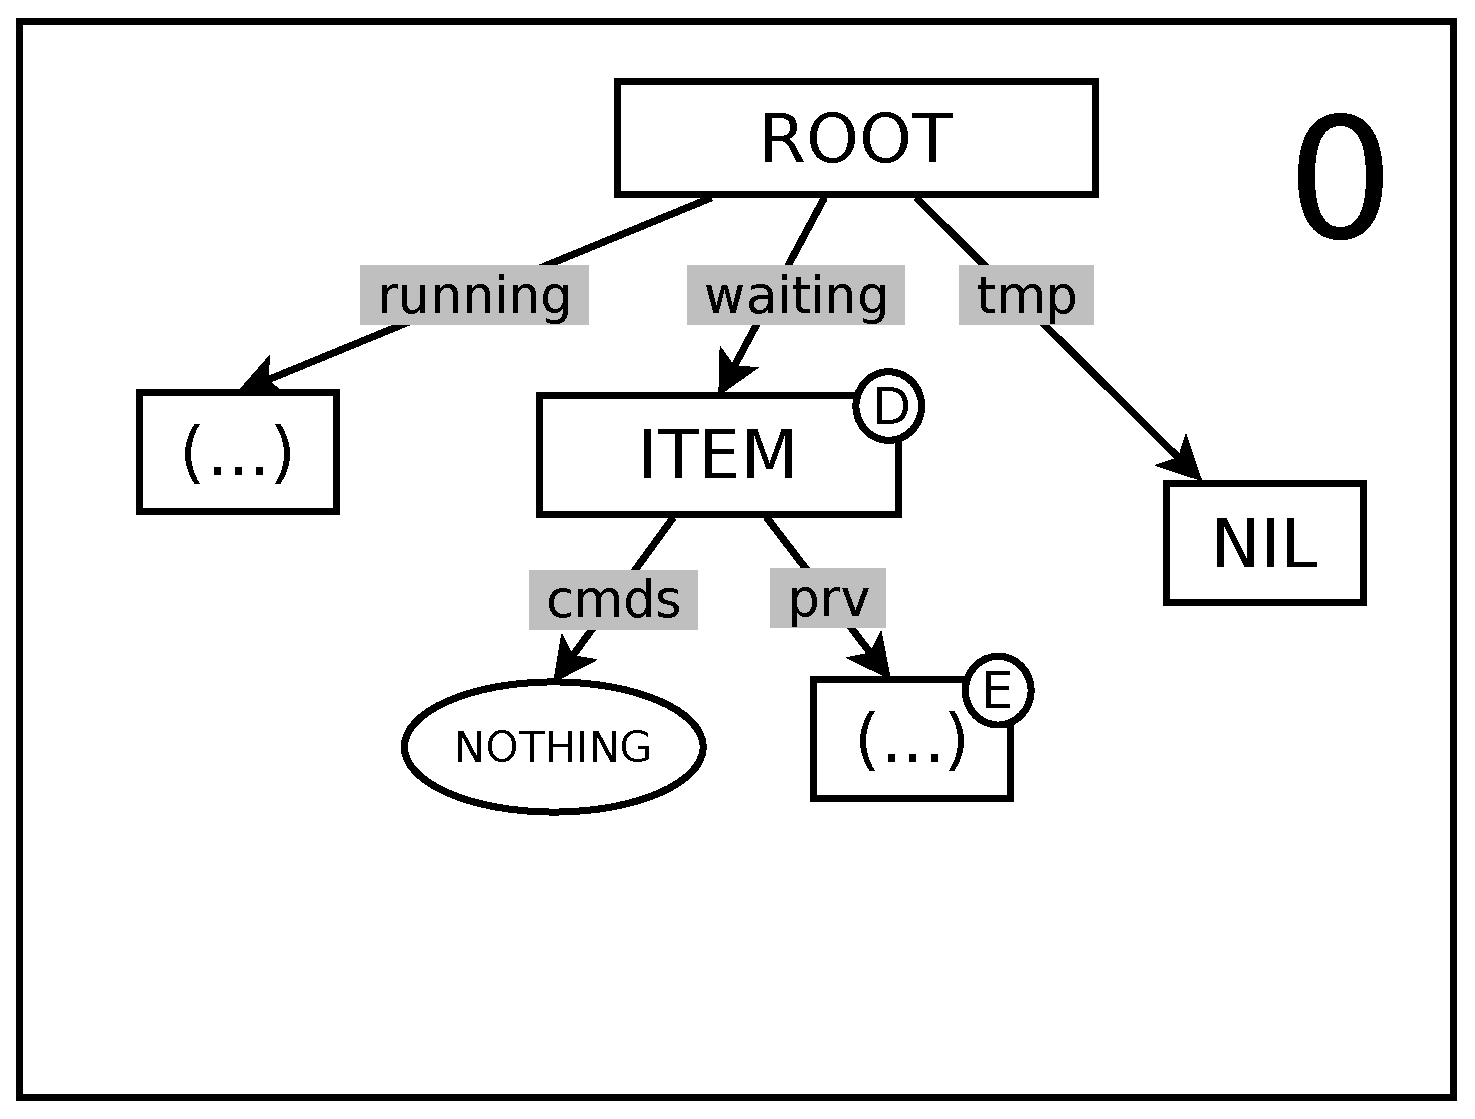
\includegraphics[scale=0.23]{queue-20.eps}
\end{minipage}

\begin{minipage}[t]{0.99\linewidth}
\centering
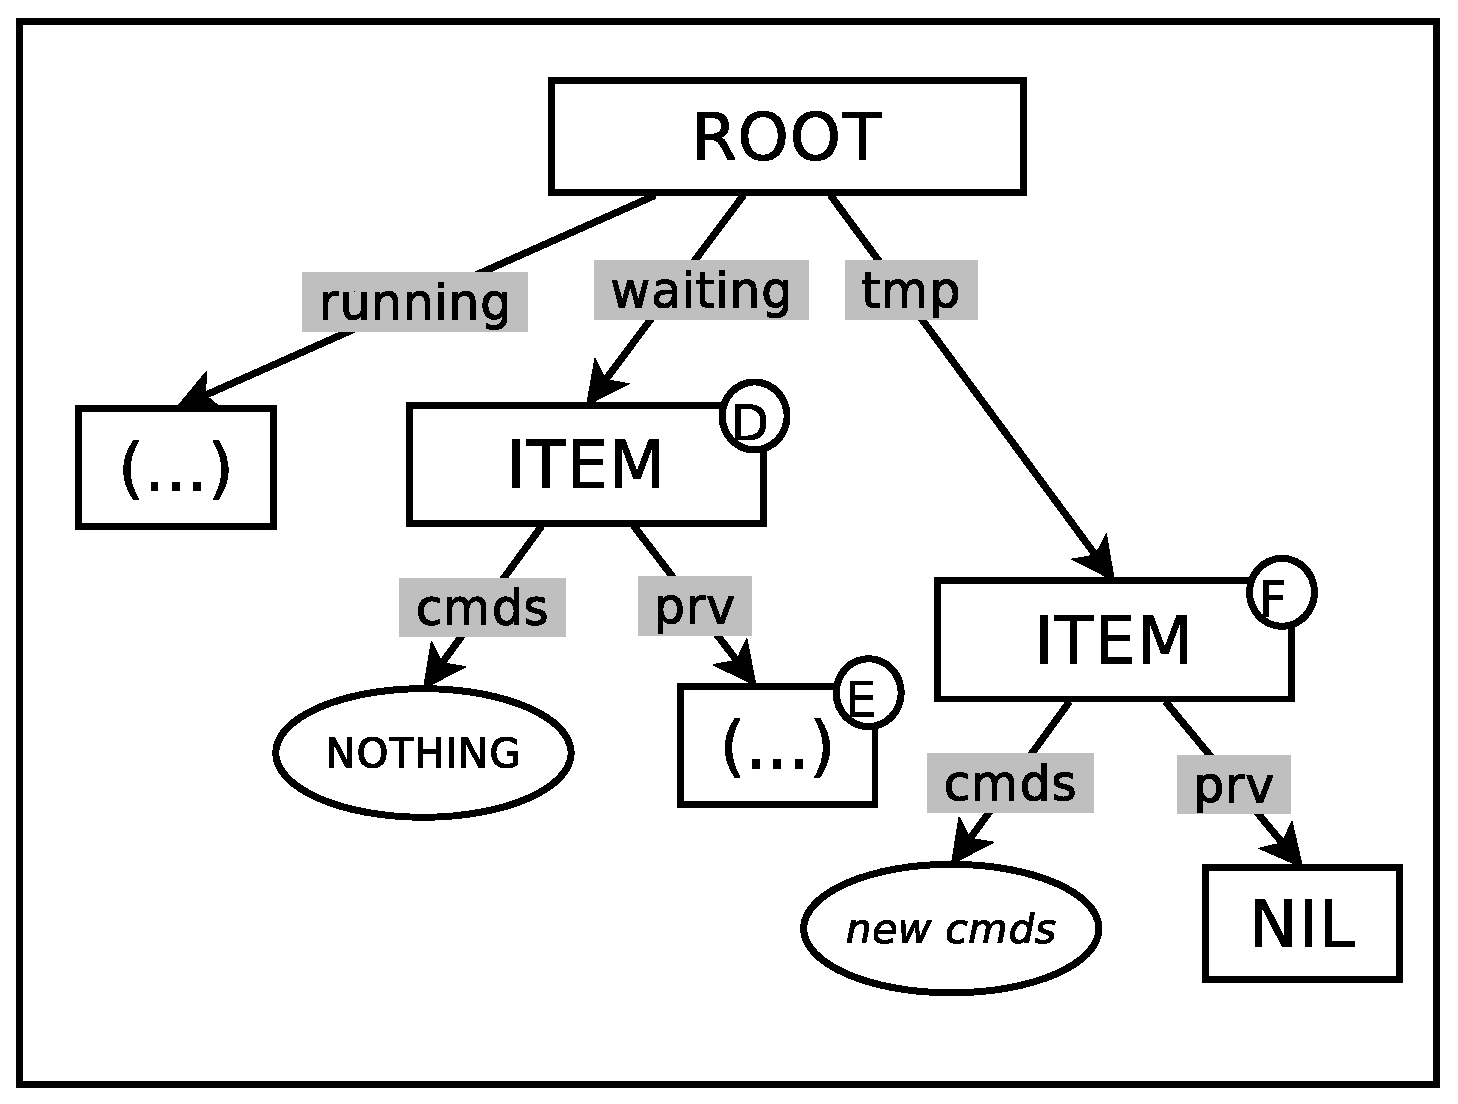
\includegraphics[scale=0.23]{queue-21.eps}
\end{minipage}

\begin{minipage}[t]{0.99\linewidth}
\centering
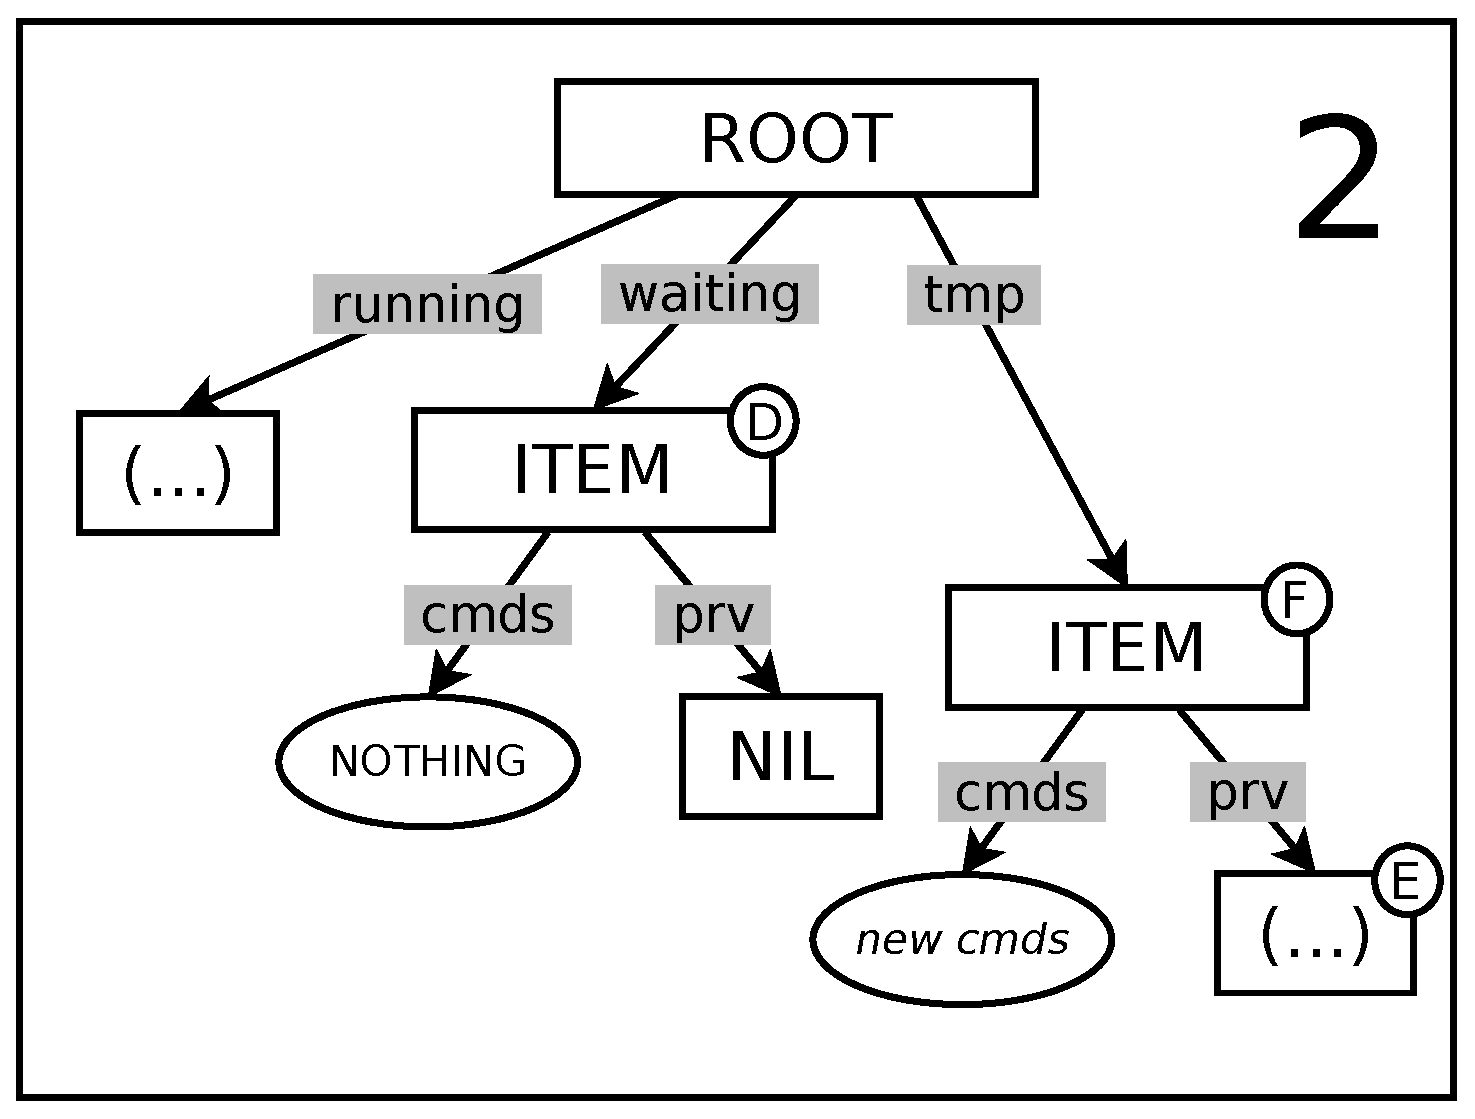
\includegraphics[scale=0.23]{queue-22.eps}
\end{minipage}

\begin{minipage}[t]{0.99\linewidth}
\centering
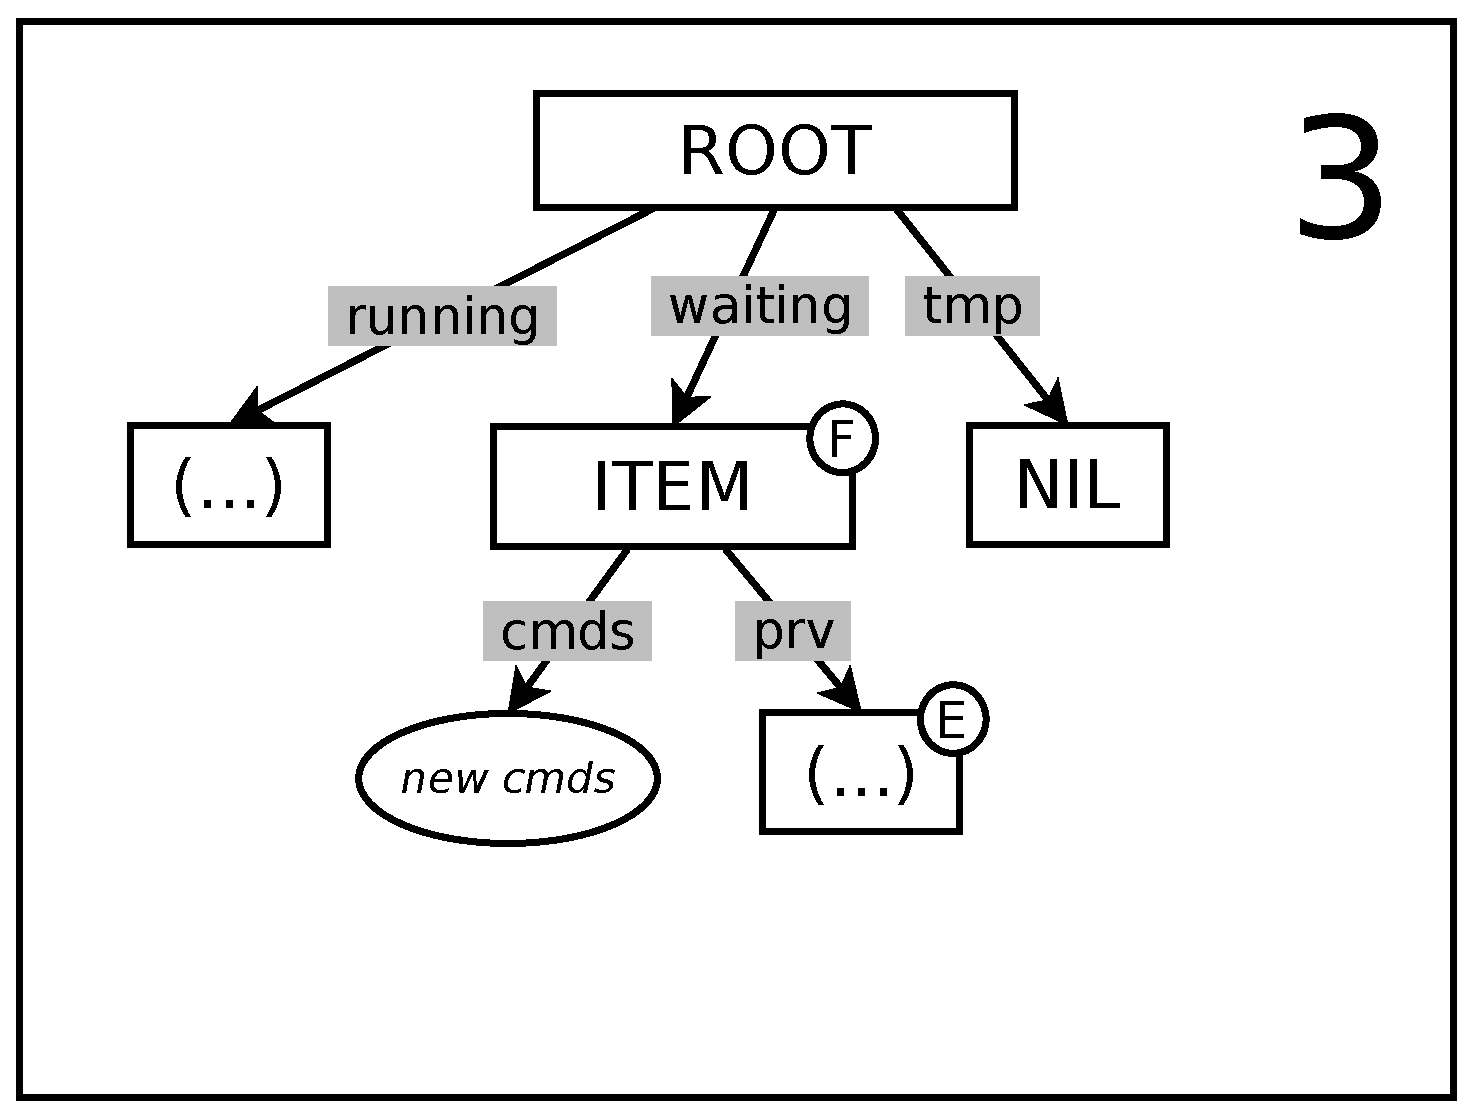
\includegraphics[scale=0.23]{queue-23.eps}
\end{minipage}
\caption{
Enqueuing new commands.
\label{fig.queue-2}
}
\end{figure}

\section{Related Work}

...

\begin{comment}
What to compare against???

Found this: http://arxiv.org/pdf/1104.2293.pdf
Follow the references.
\end{comment}

\section{Conclusion}

We presented a new construct for traversing recursive data types
incrementally, in the context of \CEU, an imperative reactive language with
synchronous concurrency. The \code{traverse} construct encapsulates an idiom
for performing recursive traversal by handling each step as a separate trail
of execution. This allows parallel traversal using the language's concurrency
features, while maintaining its safety properties.

This kind of traversal can be performed in \CEU through the use of organisms
(pooled objects which launch their own execution trails) and orthogonal
abortion via the \code{watching} construct. Combining these features to
traverse a recursive data structure correctly, however, is not straightforward.
Recursing in a way such that parallel constructs can be composed requires each
step of the recursion to be a new execution trail. Ensuring that the traversal
will not execute on a stale subtree in case the structure is modified requires
the nodes to be watched in order to perform abortions. Additionally, by
presenting a control construct that is tied to a data structure, we can ensure
bounded execution time, in line with the \CEU philosophy. By dealing with these
concerns internally in the \code{traverse} statement, we make reactive
traversal as easy to perform correctly as a recursive function call.

%TODO: mention/review other examples

\begin{comment}
Difficult because of
    multiple stack frames
    concurrent stack frames
    persistent stack frames (across reactions, with other parts executing)
    -DONE- static memory management
    -DONE- mutation of the data structure being traversed
\end{comment}

In the current implementation of recursive data types in \CEU, we impose
restrictions to the kinds of structures that can be represented. The
requirement of a tree hierarchy of ownership and move semantics for assignment
of structure fields requires care in the design of algorithms
manipulating these structures, as illustrated in Section \ref{sub.enqueuing}.
This is done to support static memory management with bounded memory pools for
allocation and deterministic deallocation. Still, we do not feel that the
restrictions are prohibitively limiting. For instance, persistent data
structures in functional languages \cite{TODO} operate under tighter design constraints.

Limitations:

- high-order programming

\bibliographystyle{abbrv}
\bibliography{rebls-15}
\balancecolumns
\end{document}
